\section{Sharp qubit frontier and its improvement}\label{sec:joint}
\begin{theorem}[Sharp joint centre--marginal bound]\label{thm:joint}
For a two-qubit state with $b<1$,
\begin{equation}\label{eq:joint}
 \boxed{f(\rho)\le\Fe(c,b)=
 \frac{\bigl[\sqrt{1+b}+\sqrt{(1-c)(1-b)}\bigr]^2}{4}.}
\end{equation}
Every pair $0\le c\le1$, $0\le b<1$ occurs and attains the bound.
\end{theorem}
\begin{proof}
The canonical Alice spectrum is $((1+c)/2,(1-c)/2)$; the physical Bob spectrum is $((1+b)/2,(1-b)/2)$. Substitute these in Theorem~\ref{thm:canonical-spectra}.

An attaining state is
\begin{equation}\label{eq:joint-state}
 \rho_{c,b}=\frac12\ket{v_{c,b}}\bra{v_{c,b}}+
 \frac{c(1-b)}2\ket{01}\bra{01},\quad
 \ket{v_{c,b}}=\sqrt{1+b}\ket{00}+\sqrt{(1-c)(1-b)}\ket{11}.
\end{equation}
It is positive and has trace one. Direct calculation gives
\begin{align*}
 a_z&=c+(1-c)b,& b_z&=b,\\
 T_{xx}&=\sqrt{(1-c)(1-b^2)},&T_{yy}&=-T_{xx},&T_{zz}&=1-c+cb,
\end{align*}
with all other Bloch and correlation coordinates zero. Thus $(\bm a-T\bm b)/(1-b^2)=c\bm e_z$. Its overlap with $\Phi^+=(\ket{00}+\ket{11})/\sqrt2$ is exactly $\Fe(c,b)$. The universal upper bound makes this its actual FEF.\end{proof}

\begin{figure}[ht]\centering
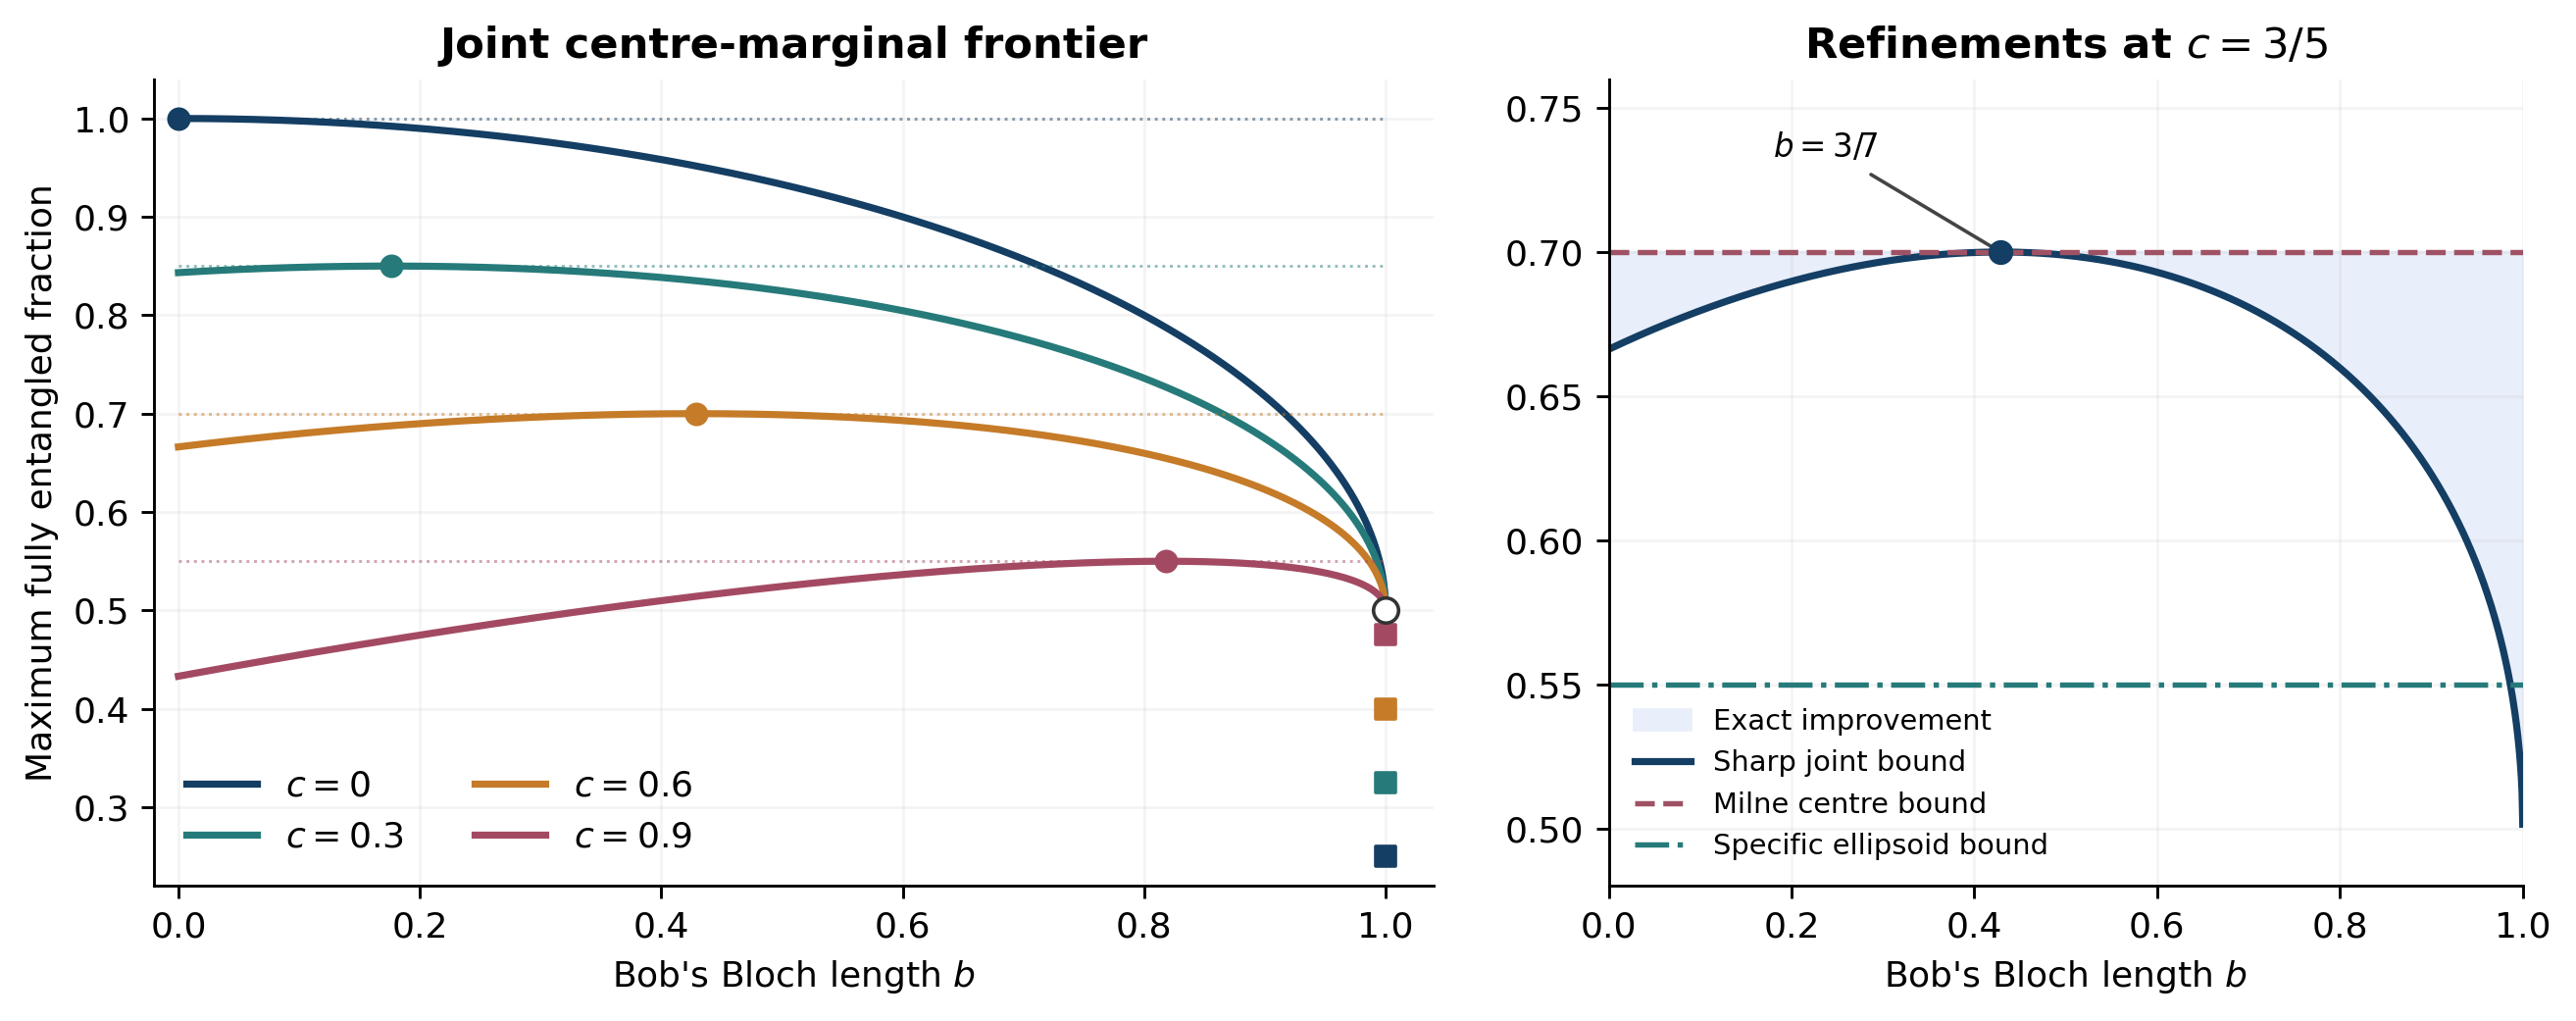
\includegraphics[width=\textwidth]{sharp_frontier.png}
\caption{Left: the exact frontier for $b<1$. Dots mark the centre-only maxima; squares give the distinct exact values on the singular $b=1$ stratum. The open endpoint marks the $b\to1^-$ limit. Right: joint and shape refinements at $c=3/5$; the shape line applies to the specific ellipsoid of Section~\ref{sec:shape}, not to every state with that centre.}
\end{figure}

The exact improvement over Milne's inequality is
\begin{equation}\label{eq:deficit}
 \boxed{1-\frac c2-\Fe(c,b)=
 \frac{\bigl[\sqrt{1-b}-\sqrt{(1-c)(1+b)}\bigr]^2}{4}.}
\end{equation}
Consequently $\Fe(c,b)\le1-c/2$, with equality if and only if
\begin{equation}\label{eq:boptimal}
 b=\frac{c}{2-c}.
\end{equation}
At $b=0$, \eqref{eq:joint} reduces to Milne's established canonical-state theorem
\[
 \Fe(c,0)=\frac{(1+\sqrt{1-c})^2}{4}.
\]
The joint theorem therefore interpolates two previously separate bounds, and proves a strict improvement whenever $b\ne c/(2-c)$.

If $\varepsilon=1-c/2-f(\rho)$, then
\begin{equation}\label{eq:qubit-stability}
 \left|b-\frac{c}{2-c}\right|^2\le\frac{8\varepsilon}{2-c}.
\end{equation}
One way to see this is the $d=2$ instance of \eqref{eq:highdim-stability}. Alternatively rationalize the difference in \eqref{eq:deficit} and use
\[
 \bigl[\sqrt{1-b}+\sqrt{(1-c)(1+b)}\bigr]^2\le2(2-c).
\]
The exact identity, unique value \eqref{eq:boptimal}, and inequality \eqref{eq:qubit-stability} are checked in Lean.

